% Created by tikzDevice version 0.12.3.1 on 2020-11-19 19:59:03
% !TEX encoding = UTF-8 Unicode
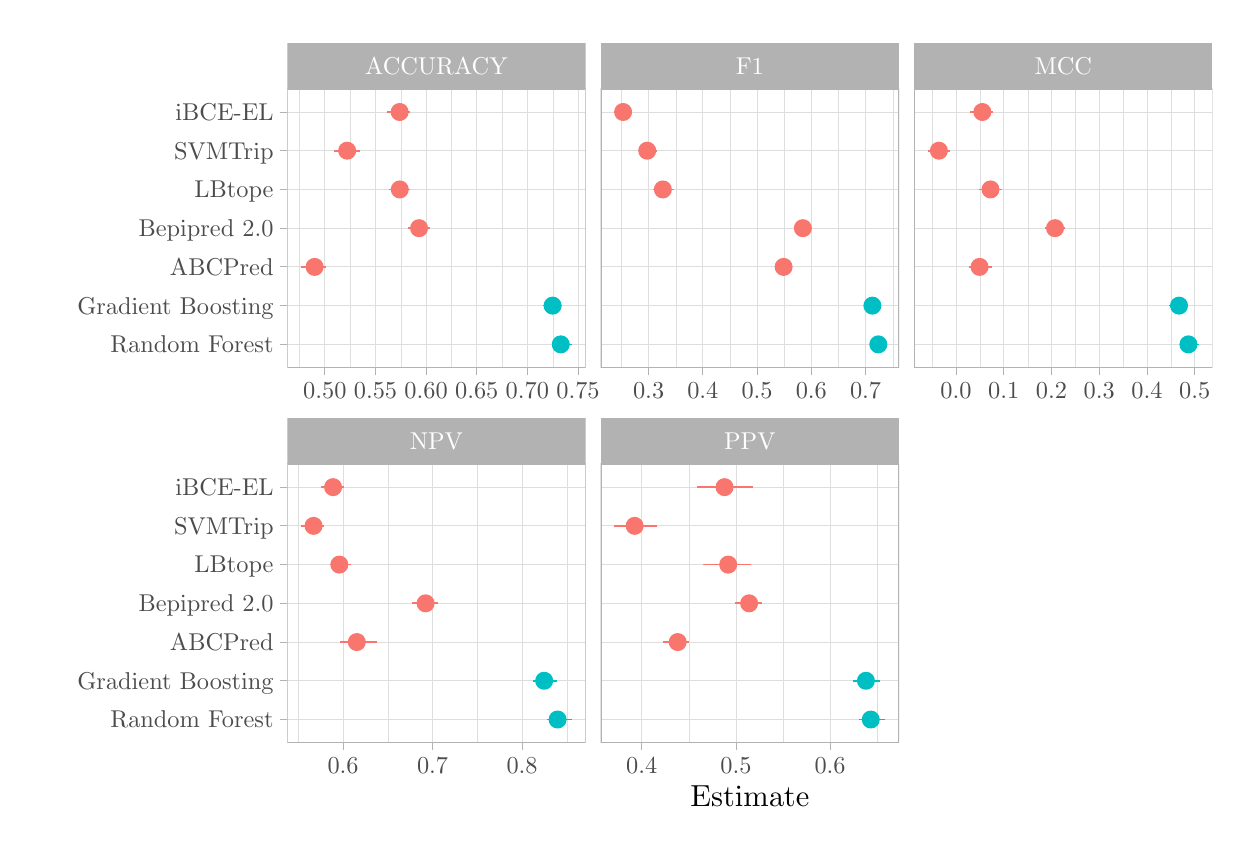
\begin{tikzpicture}[x=1pt,y=1pt]
\definecolor{fillColor}{RGB}{255,255,255}
\path[use as bounding box,fill=fillColor,fill opacity=0.00] (0,0) rectangle (433.62,289.08);
\begin{scope}
\path[clip] (  0.00,  0.00) rectangle (433.62,289.08);
\definecolor{drawColor}{RGB}{255,255,255}
\definecolor{fillColor}{RGB}{255,255,255}

\path[draw=drawColor,line width= 0.6pt,line join=round,line cap=round,fill=fillColor] (  0.00,  0.00) rectangle (433.62,289.08);
\end{scope}
\begin{scope}
\path[clip] ( 93.80,166.24) rectangle (201.57,267.01);
\definecolor{fillColor}{RGB}{255,255,255}

\path[fill=fillColor] ( 93.80,166.24) rectangle (201.57,267.01);
\definecolor{drawColor}{gray}{0.87}

\path[draw=drawColor,line width= 0.1pt,line join=round] ( 98.24,166.24) --
	( 98.24,267.01);

\path[draw=drawColor,line width= 0.1pt,line join=round] (116.54,166.24) --
	(116.54,267.01);

\path[draw=drawColor,line width= 0.1pt,line join=round] (134.83,166.24) --
	(134.83,267.01);

\path[draw=drawColor,line width= 0.1pt,line join=round] (153.13,166.24) --
	(153.13,267.01);

\path[draw=drawColor,line width= 0.1pt,line join=round] (171.42,166.24) --
	(171.42,267.01);

\path[draw=drawColor,line width= 0.1pt,line join=round] (189.72,166.24) --
	(189.72,267.01);

\path[draw=drawColor,line width= 0.3pt,line join=round] ( 93.80,174.64) --
	(201.57,174.64);

\path[draw=drawColor,line width= 0.3pt,line join=round] ( 93.80,188.64) --
	(201.57,188.64);

\path[draw=drawColor,line width= 0.3pt,line join=round] ( 93.80,202.63) --
	(201.57,202.63);

\path[draw=drawColor,line width= 0.3pt,line join=round] ( 93.80,216.63) --
	(201.57,216.63);

\path[draw=drawColor,line width= 0.3pt,line join=round] ( 93.80,230.62) --
	(201.57,230.62);

\path[draw=drawColor,line width= 0.3pt,line join=round] ( 93.80,244.62) --
	(201.57,244.62);

\path[draw=drawColor,line width= 0.3pt,line join=round] ( 93.80,258.61) --
	(201.57,258.61);

\path[draw=drawColor,line width= 0.3pt,line join=round] (107.39,166.24) --
	(107.39,267.01);

\path[draw=drawColor,line width= 0.3pt,line join=round] (125.69,166.24) --
	(125.69,267.01);

\path[draw=drawColor,line width= 0.3pt,line join=round] (143.98,166.24) --
	(143.98,267.01);

\path[draw=drawColor,line width= 0.3pt,line join=round] (162.28,166.24) --
	(162.28,267.01);

\path[draw=drawColor,line width= 0.3pt,line join=round] (180.57,166.24) --
	(180.57,267.01);

\path[draw=drawColor,line width= 0.3pt,line join=round] (198.87,166.24) --
	(198.87,267.01);
\definecolor{drawColor}{RGB}{0,191,196}

\path[draw=drawColor,line width= 0.6pt,line join=round] (189.37,174.64) -- (196.67,174.64);

\path[draw=drawColor,line width= 0.6pt,line join=round] (186.19,188.64) -- (192.99,188.64);
\definecolor{drawColor}{RGB}{248,118,109}

\path[draw=drawColor,line width= 0.6pt,line join=round] ( 98.70,202.63) -- (107.86,202.63);

\path[draw=drawColor,line width= 0.6pt,line join=round] (137.55,216.63) -- (145.38,216.63);

\path[draw=drawColor,line width= 0.6pt,line join=round] (130.47,230.62) -- (138.31,230.62);

\path[draw=drawColor,line width= 0.6pt,line join=round] (110.69,244.62) -- (119.92,244.62);

\path[draw=drawColor,line width= 0.6pt,line join=round] (129.79,258.61) -- (138.27,258.61);
\definecolor{drawColor}{RGB}{0,191,196}
\definecolor{fillColor}{RGB}{0,191,196}

\path[draw=drawColor,line width= 0.8pt,line join=round,line cap=round,fill=fillColor] (192.63,174.64) circle (  2.85);

\path[draw=drawColor,line width= 0.8pt,line join=round,line cap=round,fill=fillColor] (189.69,188.64) circle (  2.85);
\definecolor{drawColor}{RGB}{248,118,109}
\definecolor{fillColor}{RGB}{248,118,109}

\path[draw=drawColor,line width= 0.8pt,line join=round,line cap=round,fill=fillColor] (103.68,202.63) circle (  2.85);

\path[draw=drawColor,line width= 0.8pt,line join=round,line cap=round,fill=fillColor] (141.42,216.63) circle (  2.85);

\path[draw=drawColor,line width= 0.8pt,line join=round,line cap=round,fill=fillColor] (134.46,230.62) circle (  2.85);

\path[draw=drawColor,line width= 0.8pt,line join=round,line cap=round,fill=fillColor] (115.44,244.62) circle (  2.85);

\path[draw=drawColor,line width= 0.8pt,line join=round,line cap=round,fill=fillColor] (134.42,258.61) circle (  2.85);
\definecolor{drawColor}{gray}{0.70}

\path[draw=drawColor,line width= 0.6pt,line join=round,line cap=round] ( 93.80,166.24) rectangle (201.57,267.01);
\end{scope}
\begin{scope}
\path[clip] ( 93.80, 30.69) rectangle (201.57,131.45);
\definecolor{fillColor}{RGB}{255,255,255}

\path[fill=fillColor] ( 93.80, 30.69) rectangle (201.57,131.45);
\definecolor{drawColor}{gray}{0.87}

\path[draw=drawColor,line width= 0.1pt,line join=round] ( 97.80, 30.69) --
	( 97.80,131.45);

\path[draw=drawColor,line width= 0.1pt,line join=round] (130.14, 30.69) --
	(130.14,131.45);

\path[draw=drawColor,line width= 0.1pt,line join=round] (162.48, 30.69) --
	(162.48,131.45);

\path[draw=drawColor,line width= 0.1pt,line join=round] (194.82, 30.69) --
	(194.82,131.45);

\path[draw=drawColor,line width= 0.3pt,line join=round] ( 93.80, 39.08) --
	(201.57, 39.08);

\path[draw=drawColor,line width= 0.3pt,line join=round] ( 93.80, 53.08) --
	(201.57, 53.08);

\path[draw=drawColor,line width= 0.3pt,line join=round] ( 93.80, 67.07) --
	(201.57, 67.07);

\path[draw=drawColor,line width= 0.3pt,line join=round] ( 93.80, 81.07) --
	(201.57, 81.07);

\path[draw=drawColor,line width= 0.3pt,line join=round] ( 93.80, 95.06) --
	(201.57, 95.06);

\path[draw=drawColor,line width= 0.3pt,line join=round] ( 93.80,109.06) --
	(201.57,109.06);

\path[draw=drawColor,line width= 0.3pt,line join=round] ( 93.80,123.05) --
	(201.57,123.05);

\path[draw=drawColor,line width= 0.3pt,line join=round] (113.97, 30.69) --
	(113.97,131.45);

\path[draw=drawColor,line width= 0.3pt,line join=round] (146.31, 30.69) --
	(146.31,131.45);

\path[draw=drawColor,line width= 0.3pt,line join=round] (178.65, 30.69) --
	(178.65,131.45);
\definecolor{drawColor}{RGB}{0,191,196}

\path[draw=drawColor,line width= 0.6pt,line join=round] (187.79, 39.08) -- (196.67, 39.08);

\path[draw=drawColor,line width= 0.6pt,line join=round] (182.43, 53.08) -- (191.43, 53.08);
\definecolor{drawColor}{RGB}{248,118,109}

\path[draw=drawColor,line width= 0.6pt,line join=round] (112.94, 67.07) -- (126.09, 67.07);

\path[draw=drawColor,line width= 0.6pt,line join=round] (139.03, 81.07) -- (148.43, 81.07);

\path[draw=drawColor,line width= 0.6pt,line join=round] (109.12, 95.06) -- (116.87, 95.06);

\path[draw=drawColor,line width= 0.6pt,line join=round] ( 98.70,109.06) -- (106.94,109.06);

\path[draw=drawColor,line width= 0.6pt,line join=round] (106.10,123.05) -- (114.36,123.05);
\definecolor{drawColor}{RGB}{0,191,196}
\definecolor{fillColor}{RGB}{0,191,196}

\path[draw=drawColor,line width= 0.8pt,line join=round,line cap=round,fill=fillColor] (191.49, 39.08) circle (  2.85);

\path[draw=drawColor,line width= 0.8pt,line join=round,line cap=round,fill=fillColor] (186.63, 53.08) circle (  2.85);
\definecolor{drawColor}{RGB}{248,118,109}
\definecolor{fillColor}{RGB}{248,118,109}

\path[draw=drawColor,line width= 0.8pt,line join=round,line cap=round,fill=fillColor] (118.93, 67.07) circle (  2.85);

\path[draw=drawColor,line width= 0.8pt,line join=round,line cap=round,fill=fillColor] (143.79, 81.07) circle (  2.85);

\path[draw=drawColor,line width= 0.8pt,line join=round,line cap=round,fill=fillColor] (112.62, 95.06) circle (  2.85);

\path[draw=drawColor,line width= 0.8pt,line join=round,line cap=round,fill=fillColor] (103.30,109.06) circle (  2.85);

\path[draw=drawColor,line width= 0.8pt,line join=round,line cap=round,fill=fillColor] (110.35,123.05) circle (  2.85);
\definecolor{drawColor}{gray}{0.70}

\path[draw=drawColor,line width= 0.6pt,line join=round,line cap=round] ( 93.80, 30.69) rectangle (201.57,131.45);
\end{scope}
\begin{scope}
\path[clip] (207.07,166.24) rectangle (314.85,267.01);
\definecolor{fillColor}{RGB}{255,255,255}

\path[fill=fillColor] (207.07,166.24) rectangle (314.85,267.01);
\definecolor{drawColor}{gray}{0.87}

\path[draw=drawColor,line width= 0.1pt,line join=round] (214.58,166.24) --
	(214.58,267.01);

\path[draw=drawColor,line width= 0.1pt,line join=round] (234.18,166.24) --
	(234.18,267.01);

\path[draw=drawColor,line width= 0.1pt,line join=round] (253.78,166.24) --
	(253.78,267.01);

\path[draw=drawColor,line width= 0.1pt,line join=round] (273.38,166.24) --
	(273.38,267.01);

\path[draw=drawColor,line width= 0.1pt,line join=round] (292.98,166.24) --
	(292.98,267.01);

\path[draw=drawColor,line width= 0.1pt,line join=round] (312.58,166.24) --
	(312.58,267.01);

\path[draw=drawColor,line width= 0.3pt,line join=round] (207.07,174.64) --
	(314.85,174.64);

\path[draw=drawColor,line width= 0.3pt,line join=round] (207.07,188.64) --
	(314.85,188.64);

\path[draw=drawColor,line width= 0.3pt,line join=round] (207.07,202.63) --
	(314.85,202.63);

\path[draw=drawColor,line width= 0.3pt,line join=round] (207.07,216.63) --
	(314.85,216.63);

\path[draw=drawColor,line width= 0.3pt,line join=round] (207.07,230.62) --
	(314.85,230.62);

\path[draw=drawColor,line width= 0.3pt,line join=round] (207.07,244.62) --
	(314.85,244.62);

\path[draw=drawColor,line width= 0.3pt,line join=round] (207.07,258.61) --
	(314.85,258.61);

\path[draw=drawColor,line width= 0.3pt,line join=round] (224.38,166.24) --
	(224.38,267.01);

\path[draw=drawColor,line width= 0.3pt,line join=round] (243.98,166.24) --
	(243.98,267.01);

\path[draw=drawColor,line width= 0.3pt,line join=round] (263.58,166.24) --
	(263.58,267.01);

\path[draw=drawColor,line width= 0.3pt,line join=round] (283.18,166.24) --
	(283.18,267.01);

\path[draw=drawColor,line width= 0.3pt,line join=round] (302.78,166.24) --
	(302.78,267.01);
\definecolor{drawColor}{RGB}{0,191,196}

\path[draw=drawColor,line width= 0.6pt,line join=round] (305.03,174.64) -- (309.95,174.64);

\path[draw=drawColor,line width= 0.6pt,line join=round] (302.55,188.64) -- (307.51,188.64);
\definecolor{drawColor}{RGB}{248,118,109}

\path[draw=drawColor,line width= 0.6pt,line join=round] (270.28,202.63) -- (275.35,202.63);

\path[draw=drawColor,line width= 0.6pt,line join=round] (277.68,216.63) -- (282.90,216.63);

\path[draw=drawColor,line width= 0.6pt,line join=round] (225.92,230.62) -- (233.53,230.62);

\path[draw=drawColor,line width= 0.6pt,line join=round] (220.80,244.62) -- (227.31,244.62);

\path[draw=drawColor,line width= 0.6pt,line join=round] (211.97,258.61) -- (218.25,258.61);
\definecolor{drawColor}{RGB}{0,191,196}
\definecolor{fillColor}{RGB}{0,191,196}

\path[draw=drawColor,line width= 0.8pt,line join=round,line cap=round,fill=fillColor] (307.38,174.64) circle (  2.85);

\path[draw=drawColor,line width= 0.8pt,line join=round,line cap=round,fill=fillColor] (305.24,188.64) circle (  2.85);
\definecolor{drawColor}{RGB}{248,118,109}
\definecolor{fillColor}{RGB}{248,118,109}

\path[draw=drawColor,line width= 0.8pt,line join=round,line cap=round,fill=fillColor] (273.15,202.63) circle (  2.85);

\path[draw=drawColor,line width= 0.8pt,line join=round,line cap=round,fill=fillColor] (280.11,216.63) circle (  2.85);

\path[draw=drawColor,line width= 0.8pt,line join=round,line cap=round,fill=fillColor] (229.52,230.62) circle (  2.85);

\path[draw=drawColor,line width= 0.8pt,line join=round,line cap=round,fill=fillColor] (223.87,244.62) circle (  2.85);

\path[draw=drawColor,line width= 0.8pt,line join=round,line cap=round,fill=fillColor] (215.16,258.61) circle (  2.85);
\definecolor{drawColor}{gray}{0.70}

\path[draw=drawColor,line width= 0.6pt,line join=round,line cap=round] (207.07,166.24) rectangle (314.85,267.01);
\end{scope}
\begin{scope}
\path[clip] (207.07, 30.69) rectangle (314.85,131.45);
\definecolor{fillColor}{RGB}{255,255,255}

\path[fill=fillColor] (207.07, 30.69) rectangle (314.85,131.45);
\definecolor{drawColor}{gray}{0.87}

\path[draw=drawColor,line width= 0.1pt,line join=round] (238.92, 30.69) --
	(238.92,131.45);

\path[draw=drawColor,line width= 0.1pt,line join=round] (272.95, 30.69) --
	(272.95,131.45);

\path[draw=drawColor,line width= 0.1pt,line join=round] (306.98, 30.69) --
	(306.98,131.45);

\path[draw=drawColor,line width= 0.3pt,line join=round] (207.07, 39.08) --
	(314.85, 39.08);

\path[draw=drawColor,line width= 0.3pt,line join=round] (207.07, 53.08) --
	(314.85, 53.08);

\path[draw=drawColor,line width= 0.3pt,line join=round] (207.07, 67.07) --
	(314.85, 67.07);

\path[draw=drawColor,line width= 0.3pt,line join=round] (207.07, 81.07) --
	(314.85, 81.07);

\path[draw=drawColor,line width= 0.3pt,line join=round] (207.07, 95.06) --
	(314.85, 95.06);

\path[draw=drawColor,line width= 0.3pt,line join=round] (207.07,109.06) --
	(314.85,109.06);

\path[draw=drawColor,line width= 0.3pt,line join=round] (207.07,123.05) --
	(314.85,123.05);

\path[draw=drawColor,line width= 0.3pt,line join=round] (221.90, 30.69) --
	(221.90,131.45);

\path[draw=drawColor,line width= 0.3pt,line join=round] (255.93, 30.69) --
	(255.93,131.45);

\path[draw=drawColor,line width= 0.3pt,line join=round] (289.96, 30.69) --
	(289.96,131.45);
\definecolor{drawColor}{RGB}{0,191,196}

\path[draw=drawColor,line width= 0.6pt,line join=round] (300.39, 39.08) -- (309.95, 39.08);

\path[draw=drawColor,line width= 0.6pt,line join=round] (298.05, 53.08) -- (307.96, 53.08);
\definecolor{drawColor}{RGB}{248,118,109}

\path[draw=drawColor,line width= 0.6pt,line join=round] (229.68, 67.07) -- (239.06, 67.07);

\path[draw=drawColor,line width= 0.6pt,line join=round] (255.67, 81.07) -- (265.27, 81.07);

\path[draw=drawColor,line width= 0.6pt,line join=round] (244.15, 95.06) -- (261.28, 95.06);

\path[draw=drawColor,line width= 0.6pt,line join=round] (211.97,109.06) -- (227.52,109.06);

\path[draw=drawColor,line width= 0.6pt,line join=round] (241.84,123.05) -- (261.97,123.05);
\definecolor{drawColor}{RGB}{0,191,196}
\definecolor{fillColor}{RGB}{0,191,196}

\path[draw=drawColor,line width= 0.8pt,line join=round,line cap=round,fill=fillColor] (304.65, 39.08) circle (  2.85);

\path[draw=drawColor,line width= 0.8pt,line join=round,line cap=round,fill=fillColor] (302.90, 53.08) circle (  2.85);
\definecolor{drawColor}{RGB}{248,118,109}
\definecolor{fillColor}{RGB}{248,118,109}

\path[draw=drawColor,line width= 0.8pt,line join=round,line cap=round,fill=fillColor] (234.89, 67.07) circle (  2.85);

\path[draw=drawColor,line width= 0.8pt,line join=round,line cap=round,fill=fillColor] (260.69, 81.07) circle (  2.85);

\path[draw=drawColor,line width= 0.8pt,line join=round,line cap=round,fill=fillColor] (253.13, 95.06) circle (  2.85);

\path[draw=drawColor,line width= 0.8pt,line join=round,line cap=round,fill=fillColor] (219.33,109.06) circle (  2.85);

\path[draw=drawColor,line width= 0.8pt,line join=round,line cap=round,fill=fillColor] (251.81,123.05) circle (  2.85);
\definecolor{drawColor}{gray}{0.70}

\path[draw=drawColor,line width= 0.6pt,line join=round,line cap=round] (207.07, 30.69) rectangle (314.85,131.45);
\end{scope}
\begin{scope}
\path[clip] (320.35,166.24) rectangle (428.12,267.01);
\definecolor{fillColor}{RGB}{255,255,255}

\path[fill=fillColor] (320.35,166.24) rectangle (428.12,267.01);
\definecolor{drawColor}{gray}{0.87}

\path[draw=drawColor,line width= 0.1pt,line join=round] (326.85,166.24) --
	(326.85,267.01);

\path[draw=drawColor,line width= 0.1pt,line join=round] (344.09,166.24) --
	(344.09,267.01);

\path[draw=drawColor,line width= 0.1pt,line join=round] (361.34,166.24) --
	(361.34,267.01);

\path[draw=drawColor,line width= 0.1pt,line join=round] (378.58,166.24) --
	(378.58,267.01);

\path[draw=drawColor,line width= 0.1pt,line join=round] (395.83,166.24) --
	(395.83,267.01);

\path[draw=drawColor,line width= 0.1pt,line join=round] (413.07,166.24) --
	(413.07,267.01);

\path[draw=drawColor,line width= 0.3pt,line join=round] (320.35,174.64) --
	(428.12,174.64);

\path[draw=drawColor,line width= 0.3pt,line join=round] (320.35,188.64) --
	(428.12,188.64);

\path[draw=drawColor,line width= 0.3pt,line join=round] (320.35,202.63) --
	(428.12,202.63);

\path[draw=drawColor,line width= 0.3pt,line join=round] (320.35,216.63) --
	(428.12,216.63);

\path[draw=drawColor,line width= 0.3pt,line join=round] (320.35,230.62) --
	(428.12,230.62);

\path[draw=drawColor,line width= 0.3pt,line join=round] (320.35,244.62) --
	(428.12,244.62);

\path[draw=drawColor,line width= 0.3pt,line join=round] (320.35,258.61) --
	(428.12,258.61);

\path[draw=drawColor,line width= 0.3pt,line join=round] (335.47,166.24) --
	(335.47,267.01);

\path[draw=drawColor,line width= 0.3pt,line join=round] (352.72,166.24) --
	(352.72,267.01);

\path[draw=drawColor,line width= 0.3pt,line join=round] (369.96,166.24) --
	(369.96,267.01);

\path[draw=drawColor,line width= 0.3pt,line join=round] (387.21,166.24) --
	(387.21,267.01);

\path[draw=drawColor,line width= 0.3pt,line join=round] (404.45,166.24) --
	(404.45,267.01);

\path[draw=drawColor,line width= 0.3pt,line join=round] (421.70,166.24) --
	(421.70,267.01);
\definecolor{drawColor}{RGB}{0,191,196}

\path[draw=drawColor,line width= 0.6pt,line join=round] (416.34,174.64) -- (423.22,174.64);

\path[draw=drawColor,line width= 0.6pt,line join=round] (412.51,188.64) -- (419.26,188.64);
\definecolor{drawColor}{RGB}{248,118,109}

\path[draw=drawColor,line width= 0.6pt,line join=round] (340.04,202.63) -- (348.44,202.63);

\path[draw=drawColor,line width= 0.6pt,line join=round] (367.61,216.63) -- (374.84,216.63);

\path[draw=drawColor,line width= 0.6pt,line join=round] (343.73,230.62) -- (351.96,230.62);

\path[draw=drawColor,line width= 0.6pt,line join=round] (325.24,244.62) -- (333.20,244.62);

\path[draw=drawColor,line width= 0.6pt,line join=round] (340.64,258.61) -- (348.83,258.61);
\definecolor{drawColor}{RGB}{0,191,196}
\definecolor{fillColor}{RGB}{0,191,196}

\path[draw=drawColor,line width= 0.8pt,line join=round,line cap=round,fill=fillColor] (419.44,174.64) circle (  2.85);

\path[draw=drawColor,line width= 0.8pt,line join=round,line cap=round,fill=fillColor] (416.04,188.64) circle (  2.85);
\definecolor{drawColor}{RGB}{248,118,109}
\definecolor{fillColor}{RGB}{248,118,109}

\path[draw=drawColor,line width= 0.8pt,line join=round,line cap=round,fill=fillColor] (343.96,202.63) circle (  2.85);

\path[draw=drawColor,line width= 0.8pt,line join=round,line cap=round,fill=fillColor] (371.23,216.63) circle (  2.85);

\path[draw=drawColor,line width= 0.8pt,line join=round,line cap=round,fill=fillColor] (347.92,230.62) circle (  2.85);

\path[draw=drawColor,line width= 0.8pt,line join=round,line cap=round,fill=fillColor] (329.27,244.62) circle (  2.85);

\path[draw=drawColor,line width= 0.8pt,line join=round,line cap=round,fill=fillColor] (344.97,258.61) circle (  2.85);
\definecolor{drawColor}{gray}{0.70}

\path[draw=drawColor,line width= 0.6pt,line join=round,line cap=round] (320.35,166.24) rectangle (428.12,267.01);
\end{scope}
\begin{scope}
\path[clip] ( 93.80,131.45) rectangle (201.57,148.02);
\definecolor{fillColor}{gray}{0.70}

\path[fill=fillColor] ( 93.80,131.45) rectangle (201.57,148.02);
\definecolor{drawColor}{RGB}{255,255,255}

\node[text=drawColor,anchor=base,inner sep=0pt, outer sep=0pt, scale=  0.88] at (147.69,136.71) {NPV};
\end{scope}
\begin{scope}
\path[clip] (207.07,131.45) rectangle (314.85,148.02);
\definecolor{fillColor}{gray}{0.70}

\path[fill=fillColor] (207.07,131.45) rectangle (314.85,148.02);
\definecolor{drawColor}{RGB}{255,255,255}

\node[text=drawColor,anchor=base,inner sep=0pt, outer sep=0pt, scale=  0.88] at (260.96,136.71) {PPV};
\end{scope}
\begin{scope}
\path[clip] ( 93.80,267.01) rectangle (201.57,283.58);
\definecolor{fillColor}{gray}{0.70}

\path[fill=fillColor] ( 93.80,267.01) rectangle (201.57,283.58);
\definecolor{drawColor}{RGB}{255,255,255}

\node[text=drawColor,anchor=base,inner sep=0pt, outer sep=0pt, scale=  0.88] at (147.69,272.26) {ACCURACY};
\end{scope}
\begin{scope}
\path[clip] (207.07,267.01) rectangle (314.85,283.58);
\definecolor{fillColor}{gray}{0.70}

\path[fill=fillColor] (207.07,267.01) rectangle (314.85,283.58);
\definecolor{drawColor}{RGB}{255,255,255}

\node[text=drawColor,anchor=base,inner sep=0pt, outer sep=0pt, scale=  0.88] at (260.96,272.26) {F1};
\end{scope}
\begin{scope}
\path[clip] (320.35,267.01) rectangle (428.12,283.58);
\definecolor{fillColor}{gray}{0.70}

\path[fill=fillColor] (320.35,267.01) rectangle (428.12,283.58);
\definecolor{drawColor}{RGB}{255,255,255}

\node[text=drawColor,anchor=base,inner sep=0pt, outer sep=0pt, scale=  0.88] at (374.23,272.26) {MCC};
\end{scope}
\begin{scope}
\path[clip] (  0.00,  0.00) rectangle (433.62,289.08);
\definecolor{drawColor}{gray}{0.70}

\path[draw=drawColor,line width= 0.3pt,line join=round] (113.97, 27.94) --
	(113.97, 30.69);

\path[draw=drawColor,line width= 0.3pt,line join=round] (146.31, 27.94) --
	(146.31, 30.69);

\path[draw=drawColor,line width= 0.3pt,line join=round] (178.65, 27.94) --
	(178.65, 30.69);
\end{scope}
\begin{scope}
\path[clip] (  0.00,  0.00) rectangle (433.62,289.08);
\definecolor{drawColor}{gray}{0.30}

\node[text=drawColor,anchor=base,inner sep=0pt, outer sep=0pt, scale=  0.88] at (113.97, 19.68) {0.6};

\node[text=drawColor,anchor=base,inner sep=0pt, outer sep=0pt, scale=  0.88] at (146.31, 19.68) {0.7};

\node[text=drawColor,anchor=base,inner sep=0pt, outer sep=0pt, scale=  0.88] at (178.65, 19.68) {0.8};
\end{scope}
\begin{scope}
\path[clip] (  0.00,  0.00) rectangle (433.62,289.08);
\definecolor{drawColor}{gray}{0.70}

\path[draw=drawColor,line width= 0.3pt,line join=round] (221.90, 27.94) --
	(221.90, 30.69);

\path[draw=drawColor,line width= 0.3pt,line join=round] (255.93, 27.94) --
	(255.93, 30.69);

\path[draw=drawColor,line width= 0.3pt,line join=round] (289.96, 27.94) --
	(289.96, 30.69);
\end{scope}
\begin{scope}
\path[clip] (  0.00,  0.00) rectangle (433.62,289.08);
\definecolor{drawColor}{gray}{0.30}

\node[text=drawColor,anchor=base,inner sep=0pt, outer sep=0pt, scale=  0.88] at (221.90, 19.68) {0.4};

\node[text=drawColor,anchor=base,inner sep=0pt, outer sep=0pt, scale=  0.88] at (255.93, 19.68) {0.5};

\node[text=drawColor,anchor=base,inner sep=0pt, outer sep=0pt, scale=  0.88] at (289.96, 19.68) {0.6};
\end{scope}
\begin{scope}
\path[clip] (  0.00,  0.00) rectangle (433.62,289.08);
\definecolor{drawColor}{gray}{0.70}

\path[draw=drawColor,line width= 0.3pt,line join=round] (107.39,163.49) --
	(107.39,166.24);

\path[draw=drawColor,line width= 0.3pt,line join=round] (125.69,163.49) --
	(125.69,166.24);

\path[draw=drawColor,line width= 0.3pt,line join=round] (143.98,163.49) --
	(143.98,166.24);

\path[draw=drawColor,line width= 0.3pt,line join=round] (162.28,163.49) --
	(162.28,166.24);

\path[draw=drawColor,line width= 0.3pt,line join=round] (180.57,163.49) --
	(180.57,166.24);

\path[draw=drawColor,line width= 0.3pt,line join=round] (198.87,163.49) --
	(198.87,166.24);
\end{scope}
\begin{scope}
\path[clip] (  0.00,  0.00) rectangle (433.62,289.08);
\definecolor{drawColor}{gray}{0.30}

\node[text=drawColor,anchor=base,inner sep=0pt, outer sep=0pt, scale=  0.88] at (107.39,155.23) {0.50};

\node[text=drawColor,anchor=base,inner sep=0pt, outer sep=0pt, scale=  0.88] at (125.69,155.23) {0.55};

\node[text=drawColor,anchor=base,inner sep=0pt, outer sep=0pt, scale=  0.88] at (143.98,155.23) {0.60};

\node[text=drawColor,anchor=base,inner sep=0pt, outer sep=0pt, scale=  0.88] at (162.28,155.23) {0.65};

\node[text=drawColor,anchor=base,inner sep=0pt, outer sep=0pt, scale=  0.88] at (180.57,155.23) {0.70};

\node[text=drawColor,anchor=base,inner sep=0pt, outer sep=0pt, scale=  0.88] at (198.87,155.23) {0.75};
\end{scope}
\begin{scope}
\path[clip] (  0.00,  0.00) rectangle (433.62,289.08);
\definecolor{drawColor}{gray}{0.70}

\path[draw=drawColor,line width= 0.3pt,line join=round] (224.38,163.49) --
	(224.38,166.24);

\path[draw=drawColor,line width= 0.3pt,line join=round] (243.98,163.49) --
	(243.98,166.24);

\path[draw=drawColor,line width= 0.3pt,line join=round] (263.58,163.49) --
	(263.58,166.24);

\path[draw=drawColor,line width= 0.3pt,line join=round] (283.18,163.49) --
	(283.18,166.24);

\path[draw=drawColor,line width= 0.3pt,line join=round] (302.78,163.49) --
	(302.78,166.24);
\end{scope}
\begin{scope}
\path[clip] (  0.00,  0.00) rectangle (433.62,289.08);
\definecolor{drawColor}{gray}{0.30}

\node[text=drawColor,anchor=base,inner sep=0pt, outer sep=0pt, scale=  0.88] at (224.38,155.23) {0.3};

\node[text=drawColor,anchor=base,inner sep=0pt, outer sep=0pt, scale=  0.88] at (243.98,155.23) {0.4};

\node[text=drawColor,anchor=base,inner sep=0pt, outer sep=0pt, scale=  0.88] at (263.58,155.23) {0.5};

\node[text=drawColor,anchor=base,inner sep=0pt, outer sep=0pt, scale=  0.88] at (283.18,155.23) {0.6};

\node[text=drawColor,anchor=base,inner sep=0pt, outer sep=0pt, scale=  0.88] at (302.78,155.23) {0.7};
\end{scope}
\begin{scope}
\path[clip] (  0.00,  0.00) rectangle (433.62,289.08);
\definecolor{drawColor}{gray}{0.70}

\path[draw=drawColor,line width= 0.3pt,line join=round] (335.47,163.49) --
	(335.47,166.24);

\path[draw=drawColor,line width= 0.3pt,line join=round] (352.72,163.49) --
	(352.72,166.24);

\path[draw=drawColor,line width= 0.3pt,line join=round] (369.96,163.49) --
	(369.96,166.24);

\path[draw=drawColor,line width= 0.3pt,line join=round] (387.21,163.49) --
	(387.21,166.24);

\path[draw=drawColor,line width= 0.3pt,line join=round] (404.45,163.49) --
	(404.45,166.24);

\path[draw=drawColor,line width= 0.3pt,line join=round] (421.70,163.49) --
	(421.70,166.24);
\end{scope}
\begin{scope}
\path[clip] (  0.00,  0.00) rectangle (433.62,289.08);
\definecolor{drawColor}{gray}{0.30}

\node[text=drawColor,anchor=base,inner sep=0pt, outer sep=0pt, scale=  0.88] at (335.47,155.23) {0.0};

\node[text=drawColor,anchor=base,inner sep=0pt, outer sep=0pt, scale=  0.88] at (352.72,155.23) {0.1};

\node[text=drawColor,anchor=base,inner sep=0pt, outer sep=0pt, scale=  0.88] at (369.96,155.23) {0.2};

\node[text=drawColor,anchor=base,inner sep=0pt, outer sep=0pt, scale=  0.88] at (387.21,155.23) {0.3};

\node[text=drawColor,anchor=base,inner sep=0pt, outer sep=0pt, scale=  0.88] at (404.45,155.23) {0.4};

\node[text=drawColor,anchor=base,inner sep=0pt, outer sep=0pt, scale=  0.88] at (421.70,155.23) {0.5};
\end{scope}
\begin{scope}
\path[clip] (  0.00,  0.00) rectangle (433.62,289.08);
\definecolor{drawColor}{gray}{0.30}

\node[text=drawColor,anchor=base east,inner sep=0pt, outer sep=0pt, scale=  0.88] at ( 88.85,171.61) {Random Forest};

\node[text=drawColor,anchor=base east,inner sep=0pt, outer sep=0pt, scale=  0.88] at ( 88.85,185.61) {Gradient Boosting};

\node[text=drawColor,anchor=base east,inner sep=0pt, outer sep=0pt, scale=  0.88] at ( 88.85,199.60) {ABCPred};

\node[text=drawColor,anchor=base east,inner sep=0pt, outer sep=0pt, scale=  0.88] at ( 88.85,213.60) {Bepipred 2.0};

\node[text=drawColor,anchor=base east,inner sep=0pt, outer sep=0pt, scale=  0.88] at ( 88.85,227.59) {LBtope};

\node[text=drawColor,anchor=base east,inner sep=0pt, outer sep=0pt, scale=  0.88] at ( 88.85,241.59) {SVMTrip};

\node[text=drawColor,anchor=base east,inner sep=0pt, outer sep=0pt, scale=  0.88] at ( 88.85,255.58) {iBCE-EL};
\end{scope}
\begin{scope}
\path[clip] (  0.00,  0.00) rectangle (433.62,289.08);
\definecolor{drawColor}{gray}{0.70}

\path[draw=drawColor,line width= 0.3pt,line join=round] ( 91.05,174.64) --
	( 93.80,174.64);

\path[draw=drawColor,line width= 0.3pt,line join=round] ( 91.05,188.64) --
	( 93.80,188.64);

\path[draw=drawColor,line width= 0.3pt,line join=round] ( 91.05,202.63) --
	( 93.80,202.63);

\path[draw=drawColor,line width= 0.3pt,line join=round] ( 91.05,216.63) --
	( 93.80,216.63);

\path[draw=drawColor,line width= 0.3pt,line join=round] ( 91.05,230.62) --
	( 93.80,230.62);

\path[draw=drawColor,line width= 0.3pt,line join=round] ( 91.05,244.62) --
	( 93.80,244.62);

\path[draw=drawColor,line width= 0.3pt,line join=round] ( 91.05,258.61) --
	( 93.80,258.61);
\end{scope}
\begin{scope}
\path[clip] (  0.00,  0.00) rectangle (433.62,289.08);
\definecolor{drawColor}{gray}{0.30}

\node[text=drawColor,anchor=base east,inner sep=0pt, outer sep=0pt, scale=  0.88] at ( 88.85, 36.05) {Random Forest};

\node[text=drawColor,anchor=base east,inner sep=0pt, outer sep=0pt, scale=  0.88] at ( 88.85, 50.05) {Gradient Boosting};

\node[text=drawColor,anchor=base east,inner sep=0pt, outer sep=0pt, scale=  0.88] at ( 88.85, 64.04) {ABCPred};

\node[text=drawColor,anchor=base east,inner sep=0pt, outer sep=0pt, scale=  0.88] at ( 88.85, 78.04) {Bepipred 2.0};

\node[text=drawColor,anchor=base east,inner sep=0pt, outer sep=0pt, scale=  0.88] at ( 88.85, 92.03) {LBtope};

\node[text=drawColor,anchor=base east,inner sep=0pt, outer sep=0pt, scale=  0.88] at ( 88.85,106.03) {SVMTrip};

\node[text=drawColor,anchor=base east,inner sep=0pt, outer sep=0pt, scale=  0.88] at ( 88.85,120.02) {iBCE-EL};
\end{scope}
\begin{scope}
\path[clip] (  0.00,  0.00) rectangle (433.62,289.08);
\definecolor{drawColor}{gray}{0.70}

\path[draw=drawColor,line width= 0.3pt,line join=round] ( 91.05, 39.08) --
	( 93.80, 39.08);

\path[draw=drawColor,line width= 0.3pt,line join=round] ( 91.05, 53.08) --
	( 93.80, 53.08);

\path[draw=drawColor,line width= 0.3pt,line join=round] ( 91.05, 67.07) --
	( 93.80, 67.07);

\path[draw=drawColor,line width= 0.3pt,line join=round] ( 91.05, 81.07) --
	( 93.80, 81.07);

\path[draw=drawColor,line width= 0.3pt,line join=round] ( 91.05, 95.06) --
	( 93.80, 95.06);

\path[draw=drawColor,line width= 0.3pt,line join=round] ( 91.05,109.06) --
	( 93.80,109.06);

\path[draw=drawColor,line width= 0.3pt,line join=round] ( 91.05,123.05) --
	( 93.80,123.05);
\end{scope}
\begin{scope}
\path[clip] (  0.00,  0.00) rectangle (433.62,289.08);
\definecolor{drawColor}{RGB}{0,0,0}

\node[text=drawColor,anchor=base,inner sep=0pt, outer sep=0pt, scale=  1.10] at (260.96,  7.64) {Estimate};
\end{scope}
\end{tikzpicture}
